\documentclass[a4paper,12pt]{article}
\usepackage{outline}
\usepackage{pmgraph}
\usepackage[normalem]{ulem}
\usepackage{comment} % enables the use of multi-line comments (\ifx \fi)
\usepackage{lipsum} %This package just generates Lorem Ipsum filler text.
\usepackage{fullpage} % changes the margin
\usepackage{listings}
\usepackage{color}
\usepackage{mdframed}
\usepackage{listings}
\usepackage{amssymb}
\usepackage{amsmath}
\usepackage{graphicx}
\graphicspath{ {../} }
\renewcommand{\lstlistingname}{Code Block}% Listing -> Algorithm
\renewcommand{\lstlistlistingname}{List of \lstlistingname s}% List of Listings -> List of Algorithms

\linespread{1.5}
%--------------------Indention
\setlength{\parindent}{15pt}
\lstset{frame=shadowbox, rulesepcolor=\color{white}}
\mdfsetup{frametitlealignment=\center}
\lstset{
  numbers=left,
  stepnumber=1,
  firstnumber=1,
  numberfirstline=true
}

\begin{document}
\section*{Objective}

\section*{Design}

% Verilog code template
% \lstinputlisting[language=Verilog,,caption=4-Bit ALU ]{../code name.v}

\section*{Results}

% Figure with caption
% \begin{figure}[h]
%   \begin{center}
%     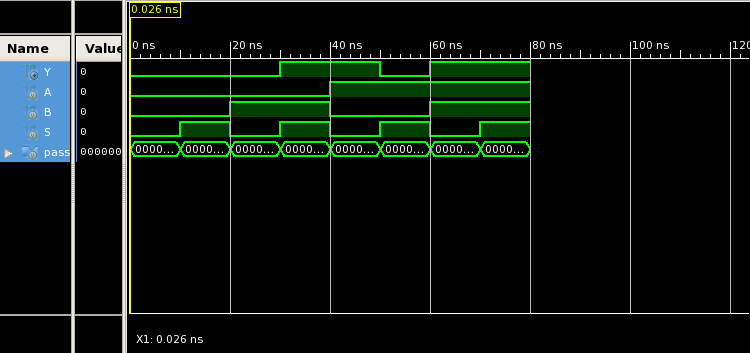
\includegraphics[scale=1]{2_1MuxPlot.png}
%     \caption{\textit{2-Bit 2:1 MUX Plots}}
%   \end{center}
% \end{figure}


\section*{Conclusion}


\section*{Questions}

\begin{enumerate}
  \item \textbf{Include the source code with comments for all modules you simulated and/or implemented in lab. You do not have to include test bench code that was provided! Code without comments will not be
accepted!}

  \item \textbf{Include screenshots of all waveforms captured during simulation in addition to the test bench console output for each test bench simulation.}

  \item \textbf{Answer all questions throughout the lab manual.}
  
  \item \textbf{A possible attack on your combination-lock is a brute-force attack in which every possible input combination is tried. Given the original design with a combination of three numbers between 0 and 19, how many possible input combinations exist? How about for the modified design with a combination of four numbers?}
\end{enumerate}

\section*{Student Feedback}

\begin{enumerate}
  \item \textbf{What did you like most about the lab assignment and why? What did you like least about it and why?}
  \vspace{10pt}

  \item \textbf{Were there any section of the lab manual that were unclear? If so, what was unclear? Do you have any suggestions for improving the clarity?}
  \vspace{10pt}

  \item \textbf{What suggestions do you have to improve the overall lab assignment?}
  \vspace{10pt}

\end{enumerate}

\ifx
\begin{thebibliography}{1}
\bibitem{Verilog} Charles Kime \& Thomas Kaminski  \emph{Logic and Computer Design Fundamentals} \\ \hspace{15pt}\textit{http://www.cs.bilkent.edu.tr/~will/courses/CS223/Verilog/LCDF3_Verilog_Ch_4.pdf}
\end{thebibliography}

\section*{Attachments}
%Make sure to change these
Lab Notes, HelloWorld.ic, FooBar.ic
%\fi %comment me out

\begin{thebibliography}{9}
\bibitem{Verilog} Charles Kime & Thomas Kaminski  \emph{Logic and Computer Design Fundamentals} \textit{http://www.cs.bilkent.edu.tr/~will/courses/CS223/Verilog/LCDF3_Verilog_Ch_4.pdf}
\end{thebibliography}

%How to cite
Put your Problem statement here! Example of a Citation\cite[p.219]{Robotics}. Here's Another Citation\cite{Flueck}
\fi
\end{document}
